% !TeX root = ../../../tesis.tex

% =====================================================================
\subsubsection{Ejemplo ilustrativo: Red Hipotética~\texorpdfstring{$\alpha$}{α}}
\label{subsubsec:garibelt-ejemplo}
% =====================================================================

La Figura~\ref{fig:garibelt-perfil-hipotetico} recorre el procedimiento
completo con la Red Hipotética~$\alpha$, cuyos valores son ilustrativos.
El perfil muestra lo que el instrumento está diseñado para detectar:
cobertura sólida en el territorio, pero eficiencia de ruta, fluidez y
distribución de carga en la banda Débil. Si esta fuera la red real de
una ciudad, el diagnóstico señalaría que el problema no es de alcance
---la red llega--- sino de calidad del servicio una vez dentro de la red.

\begin{figure}[htbp]
\centering
% Diagrama: Perfil ilustrativo — Red Hipotética α (Espectro MJG)
% Usado en: 3-Conceptos-Indicadores/3-3-Indicadores/3-3-9-Clasificacion-Garibelt/3-3-9-3-Ejemplo.tex
% fig:garibelt-perfil-hipotetico
%
% Cinco filas horizontales (una por dimensión). Fondo de bandas en tono claro,
% círculo marcador al valor normalizado, etiquetas izquierda y derecha.
% Valores de Red α: C=0.85, C_i=0.60, DI=0.40, T=0.42, B(v)=0.30
% Barra: x in [0,6]; 4 bandas en x=1.5/3.0/4.5; dy=1.0; bh=0.60

\tikzsetnextfilename{garibelt-perfil-hipotetico}
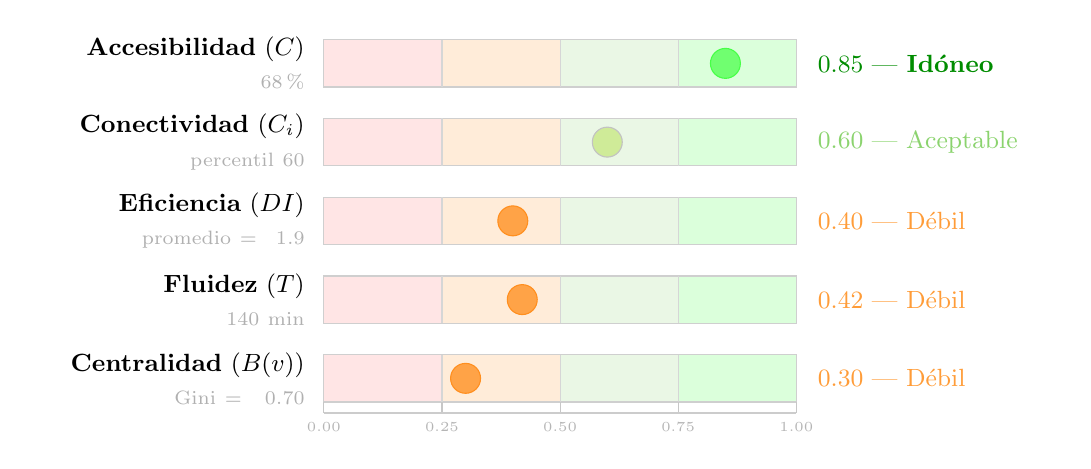
\begin{tikzpicture}[
    etiq/.style = {
        font       = \small,
        align      = right,
        text width = 3.4cm
    },
    vallab/.style = {
        font       = \small,
        align      = left,
        text width = 3.0cm,
        anchor     = west
    }
]

% ================================================================
%  FONDOS DE BANDA + BORDES (5 filas)
%  Fila n: y_base = n*1.0;  y_top = y_base + 0.60
%  Divisores de banda en x = 1.5 / 3.0 / 4.5
% ================================================================

\foreach \yb in {0, 1, 2, 3, 4}{
    \fill[red!10]              (0.0, \yb)   rectangle (1.5, \yb+0.60);
    \fill[orange!15]           (1.5, \yb)   rectangle (3.0, \yb+0.60);
    \fill[yellow!18!green!10]  (3.0, \yb)   rectangle (4.5, \yb+0.60);
    \fill[green!14]            (4.5, \yb)   rectangle (6.0, \yb+0.60);
    \draw[gray!38, thin]       (0.0, \yb)   rectangle (6.0, \yb+0.60);
    \draw[gray!32, thin]       (1.5, \yb)   -- (1.5,  \yb+0.60);
    \draw[gray!32, thin]       (3.0, \yb)   -- (3.0,  \yb+0.60);
    \draw[gray!32, thin]       (4.5, \yb)   -- (4.5,  \yb+0.60);
}

% ================================================================
%  MARCADORES (círculos rellenos con color de su banda)
%  x = valor_norm × 6 ;  y = y_base + 0.30 (centro de fila)
% ================================================================

% Fila 0 — Centralidad B(v): norm=0.30 → x=1.80 — Débil
\fill[orange!72] (1.80, 0.30) circle (0.19);
\draw[orange!88, thin] (1.80, 0.30) circle (0.19);

% Fila 1 — Fluidez T: norm=0.42 → x=2.52 — Débil
\fill[orange!72] (2.52, 1.30) circle (0.19);
\draw[orange!88, thin] (2.52, 1.30) circle (0.19);

% Fila 2 — Eficiencia DI: norm=0.40 → x=2.40 — Débil
\fill[orange!72] (2.40, 2.30) circle (0.19);
\draw[orange!88, thin] (2.40, 2.30) circle (0.19);

% Fila 3 — Conectividad C_i: norm=0.60 → x=3.60 — Aceptable
\fill[yellow!55!green!42] (3.60, 3.30) circle (0.19);
\draw[gray!48, thin] (3.60, 3.30) circle (0.19);

% Fila 4 — Accesibilidad C: norm=0.85 → x=5.10 — Idóneo
\fill[green!56] (5.10, 4.30) circle (0.19);
\draw[green!72, thin] (5.10, 4.30) circle (0.19);

% ================================================================
%  ETIQUETAS IZQUIERDA
%  dimensión (negrita) en línea 1, valor bruto en línea 2
% ================================================================

\node[etiq, anchor=east] at (-0.12, 0.30)
    {\textbf{Centralidad} ($B(v)$)\\[1pt]
     \textcolor{gray!62}{\scriptsize Gini~$= 0.70$}};

\node[etiq, anchor=east] at (-0.12, 1.30)
    {\textbf{Fluidez} ($T$)\\[1pt]
     \textcolor{gray!62}{\scriptsize 140 min}};

\node[etiq, anchor=east] at (-0.12, 2.30)
    {\textbf{Eficiencia} ($DI$)\\[1pt]
     \textcolor{gray!62}{\scriptsize promedio $= 1.9$}};

\node[etiq, anchor=east] at (-0.12, 3.30)
    {\textbf{Conectividad} ($C_i$)\\[1pt]
     \textcolor{gray!62}{\scriptsize percentil 60}};

\node[etiq, anchor=east] at (-0.12, 4.30)
    {\textbf{Accesibilidad} ($C$)\\[1pt]
     \textcolor{gray!62}{\scriptsize 68\,\%}};

% ================================================================
%  ETIQUETAS DERECHA (valor normalizado — banda)
% ================================================================

\node[vallab, color=orange!78] at (6.15, 0.30) {$0.30$ — Débil};
\node[vallab, color=orange!78] at (6.15, 1.30) {$0.42$ — Débil};
\node[vallab, color=orange!78] at (6.15, 2.30) {$0.40$ — Débil};
\node[vallab, color=yellow!30!green!65] at (6.15, 3.30) {$0.60$ — Aceptable};
\node[vallab, color=green!55!black]     at (6.15, 4.30) {$0.85$ — \textbf{Idóneo}};

% ================================================================
%  EJE DE ESCALA INFERIOR
% ================================================================

\foreach \xval/\lab in {0.0/0.00, 1.5/0.25, 3.0/0.50, 4.5/0.75, 6.0/1.00}{
    \draw[gray!44] (\xval, 0.0) -- (\xval, -0.14);
    \node[font=\tiny, color=gray!58, anchor=north] at (\xval, -0.14) {\lab};
}

% Línea de eje
\draw[gray!40] (0.0, -0.14) -- (6.0, -0.14);

\end{tikzpicture}

\caption[Perfil ilustrativo de la Clasificación Garibelt: Red Hipotética~$\alpha$]{%
    Perfil Garibelt de la Red Hipotética~$\alpha$. Cada fila corresponde a
    una dimensión del Espectro MJG; el círculo indica el valor normalizado
    y su posición en la Escala Garibelt. Los valores son ilustrativos.}
\label{fig:garibelt-perfil-hipotetico}
\fuentefigura{Elaboración propia.}
\end{figure}

De los ocho indicadores del capítulo, dos quedan fuera de la versión~1
del instrumento. $W_{s,h}$ (Penalización por Transferencia) tiene
implementación parcial en el motor \termino{VFTModel}; su incorporación
queda diferida a la versión~2. $\Delta E$ (Robustez Geométrica) requiere
múltiples corridas del grafo con nodos removidos, operación que
corresponde a la Fase~4 y está fuera del alcance del presente análisis.
La aplicación del instrumento a la red de la \zmvm{} ---incluyendo los
valores normalizados y la lectura por dimensión--- se presenta en la
\autoref{sec:diagnostico-garibelt} del \autoref{ch:analisis-red-actual}.
